 %%	SECCION documentclass																									 %%	
%%---------------------------------------------------------------------------%%
\documentclass[a4paper]{report}

%%---------------------------------------------------------------------------%%
%%	SECCION usepackage																											 %%	
%%---------------------------------------------------------------------------%%
\usepackage{amsmath, amsthm}
\usepackage[spanish,activeacute]{babel}
\usepackage{caratula}
\usepackage{a4wide}
\usepackage{hyperref}
\usepackage{fancyhdr}
\usepackage{graphicx} % Para el logo magico!
\usepackage{amssymb}
\usepackage{amsmath}
\usepackage[latin1]{inputenc}
%\usepackage [T1]{fontenc}
\usepackage[dvipsnames,usenames]{color}
\usepackage{amsfonts}
\usepackage{ulem}
%\usepackage{highlight}
\usepackage{fancybox}
%\usepackage{marvosym}
\usepackage{color}
\usepackage{lastpage}
\usepackage{lscape}
\usepackage{tabularx}

%%---------------------------------------------------------------------------%%
%%	SECCION opciones																												 %%	
%%---------------------------------------------------------------------------%%
\parskip    = 11 pt
\headheight	= 13.1pt
\pagestyle	{fancy}
\definecolor{orange}{rgb}{1,0.5,0}

\addtolength{\headwidth}{1.0in}

\addtolength{\oddsidemargin}{-0.5in}
\addtolength{\textwidth}{1.0in}
\addtolength{\topmargin}{-0.5in}
\addtolength{\textheight}{0.7in}

%%---------------------------------------------------------------------------%%
%%	SECCION document	 %%	
%%---------------------------------------------------------------------------%%
\begin{document}
\renewcommand{\chaptername}{Parte }

%%---- Caratula -------------------------------------------------------------%%
\materia{Ingenier�a del Software II (2do cuatrimestre de 2009)}
\titulo{Trabajo Pr�ctico I - Segunda Entrega}

\integrante{Castillo, Gonzalo}{164/06}{gonzalocastillo\_086@hotmail.com}
\integrante{Elizalde, Victoria}{452/06}{kivielizalde@gmail.com}
\integrante{Gonzalez, Sergio}{481/06}{gonzalezsergio2003@yahoo.com.ar}
\integrante{Page Saal, Mart�n}{315/06}{martinpage2001@yahoo.com.ar}
\resumen{
En el siguiente documento, se arribar� un sprint de Scrum intentando tambi�n de algun modo, adaptar la arquitectura a los nuevos requerimientos solicitados, para poder seguir cumpliendo los objetivos del proyecto.}

% TOC, usa estilos locos
\maketitle
\pagestyle{empty}
{
\fancypagestyle{plain}
    {
    \fancyhead{}
    \fancyfoot{}
    \renewcommand{\headrulewidth}{0.0pt}
    } % clear header and footer of plain page because of ToC
\tableofcontents
}

\newpage
% arreglos los estilos para el resto del documento, y
% reseteo los numeros de pagina para que queden bien
\pagenumbering{arabic}
\fancypagestyle{plain} {
    \fancyhead[LO]{Castillo, Elizalde, Gonzalez, Page Saal}
    \fancyhead[C]{}
    \fancyhead[RO]{P\'agina \thepage\ de \pageref{LastPage}}
    \fancyfoot{}
    \renewcommand{\headrulewidth}{0.4pt}
}
\pagestyle{plain}

\newpage
\chapter{Introducci�n}

\subsection{Notaci�n}

Agregaremos unos pocos t�rminos nuevos que se utilizaran a lo largo de este documento. 

\begin{itemize}
	\item ECP : Estaci�n Central Provincial
	\item SMP : Sistema de Monitoreo Provincial
\end{itemize}
\clearpage

\newpage
\chapter{Objetivo del sprint}

La caracter�stica principal de �ste sprint es la aparici�n de nuevos requerimientos funcionales.  Esto hace que se tenga que pensar como se adecua la arquitectura a dichos requerimientos y en caso de ser necesario, c�mo deber�a modificarse para contemplar los mismos, teniendo en cuenta que funcione todo lo hecho hasta el momento. Entonces, b�sicamente el objetivo del sprint es adaptar la arquitectura pensada en la primera entrega del trabajo pr�ctico a los nuevos requerimientos, y llevar a cabo la nueva planificaci�n utilizando scrum. Una vez hecho esto debemos seleccionar la lista de stories que llevaremos a cabo en el sprint, estimarlos (utilizando valores relativos, que luego se traducir�n a esfuerzo) y comenzar con su implementaci�n para lograr un adecuado product increment que sea aceptado por el usuario.

Ser� necesario pensar c�mo van a impactar los nuevos requerimientos en la arquitectura ya dise�ada y como realizar un adecuado trade off para seguir garantizando el cumplimiento de los antiguos requerimientos y la satisfacci�n de los nuevos.

Tambi�n se espera tener los primeros stories realizados, que se corresponden con los que se indican en el enunciado del trabajo, resolviendo los problemas que surjan en el trayecto del mismo. Este avance se ver� reflejado en el Sprint Burndown Chart final, y se podr� observar como fue evolucionando el sprint durante las 2 semanas que dura.

Se espera fijar ademas las ideas cuando se tengan dudas acerca del proyecto su avance y su desarrollo cuando tengamos las stand-up meetings correspondientes, corroborando el seguimiento del proyecto.
\clearpage


\newpage
\chapter{Planificaci�n}	


\section{Epics}

Los Epics identificados estan relacionados con los principales cambios en los requerimientos que tuvo el sistema para esta etapa. Los Epics, son similares a casos de uso, pero de muy alto nivel. Estos nos ayudar�n a agrupar tareas, que luego asignaremos a cada uno de los User Story, y poder armar los sprints, en particular el primero, que entra para esta nueva entrega del trabajo.

\begin{itemize}
\item E01 - Configurando conjunto de TRs Regionales.
\item E02 - Configurando colaboraci�n entre regiones.
\item E03 - Configurando procesamiento de modelos en forma distribuida.
\item E04 - Evaluando modelos con distintos algoritmos.
\item E05 - Suscribiendo modelos a Trs
\end{itemize}


\section{Product Backlog}

En esta secci�n se detallar�n los User Stories relacionados con los nuevos requerimientos. A su vez cada una, est� incluida dentro de alguno de los Epics descriptos anteriormente, con el objetivo de facilitar la compresion de las diferentes tareas.

\begin{itemize}

\item{US01 - E01:}\\
\begin{tabular}{|l p{12cm}|}
\hline
\textbf{Como:} & Empresa regional.\\
\textbf{Quiero:} & Estar a cargo de la parametrizaci�n ejecuci�n y resultados de mis modelos.\\
\textbf{Para:} & Trabajar de acuerdo a nuestros criterios.\\
\hline
\end{tabular}


\item{US02 - E01:}\\
\begin{tabular}{|l p{12cm}|}
\hline
\textbf{Como:} & Empresa regional.\\
\textbf{Quiero:} & Poder incorporar nuevas Tr a mi zona.\\
\textbf{Para:} & Obtener los datos necesarios para mis modelos.\\
\hline
\end{tabular}


\item{US03 - E02}\\
\begin{tabular}{|l p{12cm}|}
\hline
\textbf{Como:} & Empresa regional\\
\textbf{Quiero:} & Trabajar en colaboraci�n con otras regiones.\\
\textbf{Para:} & Poder solicitar datos  o resultados parciales procesados por los modelos de las mismas.\\
\hline
\end{tabular}


\item{US04 - E03}\\
\begin{tabular}{|l p{12cm}|}
\hline
\textbf{Como:} & Usuario del sistema.\\
\textbf{Quiero:} & Incrementar el poder de c�mputo.\\
\textbf{Para:} & Que aquellos modelos que as� lo requieran puedan llevar a cabo su procesamiento de manera �ptima.\\
\hline
\end{tabular}


\item{US05 - E01 - E02}\\
\begin{tabular}{|l p{12cm}|}
\hline
\textbf{Como:} & Usuario del sistema.\\
\textbf{Quiero:} & Atacar el incremento de congesti�n asociada a los nuevos requerimientos.\\
\textbf{Para:} & El sistema siga funcionando correctamente a tiempo sin saturar la red GSM.\\
\hline
\end{tabular}


\item{US06 - E01}\\
\begin{tabular}{|l p{12cm}|}
\hline
\textbf{Como:} & Usuario del sistema.\\
\textbf{Quiero:} & Que las terminales remotas funcionen con s�lo un subconjunto de los sensores disponibles en los casos en que as� fuese necesario.\\
\textbf{Para:} & No utilizar informaci�n innecesaria.\\
\hline
\end{tabular}


\item{US07 - E03}\\
\begin{tabular}{|l p{12cm}|}
\hline
\textbf{Como:} & Intendente.\\
\textbf{Quiero:} & Quiero que se utilicen los equipos disponibles.\\
\textbf{Para:} & Mejorar el poder de c�mputo para los modelos que as� lo requieran.\\
\hline
\end{tabular}

   
\item{US08 - E03}\\
\begin{tabular}{|l p{12cm}|}
\hline
\textbf{Como:} & Usuario del sistema.\\
\textbf{Quiero:} & Que se particionen el conjunto de reglas.\\
\textbf{Para:} & Procesarlas concurrentemente en los equipos disponibles.\\
\hline
\end{tabular}

 
\item{US09 - E03}\\
\begin{tabular}{|l p{12cm}|}
\hline
\textbf{Como:} & Usuario del Sistema.\\
\textbf{Quiero:} & Que se pueda configurar de manera sencilla la colaboraci�n entre subpartes.\\
\textbf{Para:} & Para lograr un f�cil intercambio.\\
\hline
\end{tabular}
  

\item{US010 - E03}\\
\begin{tabular}{|l p{12cm}|}
\hline
\textbf{Como:} & Usuario del Sistema.\\
\textbf{Quiero:} & Que se pueda configurar de manera sencilla la colaboraci�n entre modelos.\\
\textbf{Para:} & Para lograr un f�cil intercambio.\\
\hline
\end{tabular}


\item{US011 - E04}\\
\begin{tabular}{|l p{12cm}|}
\hline
\textbf{Como:} & Usuario del Sistema.\\
\textbf{Quiero:} & Poder tener varios algoritmos de evaluaci�n de reglas.\\
\textbf{Para:} & Para chequear consistencia de modelos.\\
\hline
\end{tabular}



\item{US012 - E05}\\
\begin{tabular}{|l p{12cm}|}
\hline
\textbf{Como:} & Usuario del Sistema.\\
\textbf{Quiero:} & Que los modelos puedan suscribirse a las TRs:\\
\textbf{Para:} & Obtener solo los datos necesarios para su procesamiento.\\
\hline
\end{tabular}

\end{itemize}
%\textbf{Como:}
%\textbf{Quiero:}
%\textbf{Para:}
%Como usuario quiero Realizar una especificaci�n clara de las modificaciones arquitect�nicas para adaptar nuestro sistema a los nuevos requerimientos.
%\textbf{Como:}
%\textbf{Quiero:}
%\textbf{Para:}
%Como usuario quiero realizar Product Backlog para tener todos los stories requeridos para realizar todo el proyecto.
%\textbf{Como:}
%\textbf{Quiero:}
%\textbf{Para:}
%Como usuario quiero realizar el Sprint Backlog  con las stories seleccionadas, su estimaci�n, criterios de aceptaci�n y descomposici�n en tareas para tener las cosas que hay que hacer para la iteraci�n actual.
%\textbf{Como:}
%\textbf{Quiero:}
%\textbf{Para:}
%Como usuario quiero realizar una documentaci�n del seguimiento de proyecto  usando burndown charts para tener una visi�n grafica del avance de la iteraci�n.
%\textbf{Como:}
%\textbf{Quiero:}
%\textbf{Para:}
%Como usuario quiero queremos realizar un dise�o de objetos para resolver el problema de la ejecuci�n de los modelos matem�ticos y puedan ser ejecutados en forma distribuida.
%\textbf{Como:}
%\textbf{Quiero:}
%\textbf{Para:}
%Como usuario quiero proyecto queremos realizar una comparaci�n del trabajo realizado con UP y SCRUM para ver las ventajas y desventajas de cada uno de las metodolog�as.
%\textbf{Como:}
%\textbf{Quiero:}
%\textbf{Para:}



\clearpage

\newpage
\chapter{Seguimiento}
En esta secci�n hablaremos sobre el seguimiento del proyecto, que se hizo bas�ndose en la metodolog�a SCRUM (como el resto del TP). SCRUM prevee un tipo de reuni�n de seguimiento: la daily stand-up meeting.

Nosotros hicimos este tipo de reuni�n informal y r�pida mas o menos constantemente a lo largo de este mes. En realidad no lo hicimos porque la metodolog�a as� lo prevee (de hecho no las hicimos todos los d�as) sino porque es algo que nos surge naturalmente del trabajo en equipo en otras materias tambi�n (hace varios a�os que hacemos grupo juntos, si bien no siempre exactamente el mismo, todos nos conoc�amos de antes). Tambi�n hicimos una reuni�n con nuestro corrector, pero esa se desvi� un poco por la presencia del mismo (aprovechamos para hacerle consultas y mostrarle lo que ten�amos).

Peri�dicamente fuimos actualizando el \textit{taskboard}, no en un pizar�n f�sico, en un archivo en nuestro repositorio. En �l �bamos cambiando el estado de las tareas y de las stories cuando era necesario: Sin empezar, en progreso, tarea terminada. Tambi�n �bamos actualizando la cantidad de horas que faltaban para terminar el proyecto. Estas horas fueron el input para armar el \textit{burndown chart}.\begin{figure}[h]
\centering
\includegraphics[scale=0.4]{./figuras/burnDown.png}
\caption{Burn Down Chart}
\end{figure}

En el burndown chart, se puede apreciar cuantas horas esfuerzo faltan para terminar el sprint. (Se puede ver esto discriminado por tareas en la tabla). Podemos ver que al principio, las horas esfuerzo se mantuvieron constantes. 

Hay dos motivos esenciales para ello: por un lado, en las stories no est�n incluidas las meta-tareas, como por ejemplo armar el product y sprint backlog, escribir los casos de aceptaci�n, o empezar a escribir este informe.

Por otro lado, al principio del trabajo pr�ctico ten�amos dudas (que iban surgiendo a medida que hac�amos las distintas partes del trabajo) que nos frenaban. Una vez que ya sab�amos exactamente que ten�amos que hacer y nos �bamos distribuyendo el trabajo espont�neamente, el ritmo de trabajo fue mayor (adem�s por la misma inercia de tener el trabajo empezado).

Los obst�culos que tuvimos fueron mas que nada temporales: la presencia del parcial de esta y de otras materias hizo que baj�ramos la cantidad de horas dedicadas al trabajo pr�ctico, pero logramos no frenar del todo el desarollo de mismo. 

Los otros obst�culos que tuvimos fue en la implementaci�n: en la primera parte del trabajo est�bamos muy contentos de haber hecho r�pidamente la implementaci�n en un lenguaje de programaci�n que ninguno dominaba. Esta vez, hubo alguno errores que nos dieron dolores de cabeza y nos hicieron pensar durante rato, pero todos fueron resueltos.

En general, estamos contentos con como se desaroll� el trabajo pr�ctico. Si bien no llegamos con tanto tiempo de sobra como hubi�ramos querido, es comprensible dado que tuvimos varias restricciones temporales (TPs y parciales de otra materia, la mitad del grupo trabaja) que hicieron que no pudi�ramos terminarlo antes.
\begin{landscape}
\begin{figure}[h]
\centering
\includegraphics[scale=0.7]{./figuras/taskboard.png}
\caption{Taskboard}
\end{figure}
\end{landscape}  
\clearpage

\newpage
\chapter{Arquitectura}

En esta parte se desarrollar� la arquitectura general del producto. Analiceremos estilos arquitect�nicos, las t�cticas correspondientes para poder contemplar los atributos de calidad y finalmente diferentes estructuras que nos conllevar�n a realizar las vistas arquitect�nicas apropiadas para lograr un buen entendimiento de las diferentes partes del sistema.

\section{Componentes y conectores}

La primera de las estructuras que vamos a analizar es la asociada a entidades run-time. Para ello utilizaremos vistas de componentes y conectores que nos permitan identificar �stas entidades y poder instanciarlas como componentes o conectores. Esto nos dar� una idea de como los diferentes componentes contribuyen a la ejecuci�n de las funcionalidades solicitadas y como las t�cticas aplicadas se corresponden al control de los diferentes atributos de calidad. Presentaremos tres vistas de acuerdo a los componentes que funcionan en cada uno de las tres grandes partes que componen nuestro sistema(Terminal Remota, Estaci�n central y Sistema de Monitoreo) y tambi�n explicaremos la forma de comunicaci�n y flujo de datos entre dichas partes. Cada una de las tres vistas se encuentran al final de �sta secci�n por lo que es aconsejable analizarla en paralelo a medida que se lee la explicaci�n del funcionamiento de las componentes internas.

\subsection{Funcionamiento de la Estaci�n Central}


\subsubsection{T�cticas elegidas en la Estaci�n Central}


\subsection{Funcionamiento del Sistema de Monitoreo}

El Sistema de Monitoreo es la parte del sistema encargada de la interfaz con los usuarios, clientes y otros sistemas externos. En este sector se prestar�n diferentes servicios, ya sea mediante una interfaz de comunicaci�n directa o mediante Web Services. Estos servicios tienen que ver, en su mayor�a, a la visualizaci�n de los datos que el sistema tenga disponible en el momento. �stos datos pueden ser:

\begin{itemize}
\item Los resultados de los m�todos procesados por la Estaci�n Central, que pueden estar destinados a clientes externos, como por ejemplo la p�gina del Ministerio de Infraestructura, o para otros clientes externos que se espera tener en un futuro, como es el caso de la empresa AgroTop.

\item Los datos que se refieren al estado general del sistema en tiempo real, el estado de la conexi�n entre las TRs y la Estaci�n central, el estado individual de cada TR, cuales de �stas est�n funcionando correctamente, cuales fueron trianguladas, y cuales no fueron trianguladas y se esta utilizando el sistema satelital Biggest Satelite para obtener los datos de su zona.

\item La informaci�n que es enviada en forma de mail a los responsables por alertas que se producen.

\item La recepci�n de datos provenientes del Sistema E�lico, que son utilizados por la Estaci�n Central para discernir que datos son mas precisos.

\end{itemize}

Como se puede observar, el Sistema de Monitoreo es la gran interfaz que tiene el sistema.

\subsubsection{Descripci�n de los componentes del Sistema de Monitoreo}

En �sta secci�n se nombrar�n y explicar�n los componentes que forman parte del Sistema de Monitoreo, asi tambi�n como su rol dentro de la arquitectura.

\begin{itemize}

\item \textbf{Interfaz SE:} Este componente es el encargado de 	comunicarse con el Sistema E�lico, implementando su protocolo de comunicaci�n, y a su vez se encarga de comunicarse con la Estaci�n Central, para enviarle los datos recibidos al componente encargado del procesamiento de los mismos.

\end{itemize}

\subsubsection{T�cticas elegidas en el Sistema de Monitoreo}


\subsection{Funcionamiento de las Terminales Remotas}


\subsubsection{T�cticas elegidas en las Terminales Remotas}


\section{Comunicaci�n entre la Estaci�n Central y el Sistema de Monitoreo}
\clearpage

\newpage
\chapter{Impediment List}

En este capitulo se mostrar� la lista $Impediment$ $List$ con los problemas que pueden surgir en el proyecto y que afecte a su productividad y calidad. Estos estar�n agrupados por los $User$ $Story$ que se realizar�n en la primera iteraci�n.

\begin{enumerate}
\item US03: Trabajar en colaboraci�n con otras regiones (modelos)

\begin{itemize}
\item Posibilidad de realizar mas cambios que lo planeado en la arquitectura para posibilitar la comunicaci�n y el intercambio de informacion.
\item Posibles problemas en la implementaci�n por uso de lenguajes o tecnicas desconocidas.
\item Aumento en el costo del testeo de los nuevos componentes y detecci�n de posibles errores en la arquitectura.
\item Equivocaci�n y falta de tiempo por pensar que era el user storie m�s sencillo.
\end{itemize}

\item US12: Suscrpci�n de modelos a Trs

\begin{itemize}
\item Problemas definiendo las interfaces y el metodo de suscripci�n de los modelos.
\item Posibilidad de realizar mas cambios que lo planeado en la arquitectura.
\item Localizaci�n de errores en la arquitectura a la hora de realizar los testeos.
\item Problemas de escalabilidad en la implementaci�n.
\item Malas estimaciones en los tiempos dado que es la tarea m�s complicada.

\end{itemize}

\item US10: Configuraci�n sencilla de colaboraci�n entre modelos
\begin{itemize}
\item Problemas para resolver la configuraci�n que permita la colaboraci�n entre modelos.
\item Localizaci�n de errores en la arquitectura a la hora de realizar los testeos.
\item Mala interpretaci�n de "sencilla".
\end{itemize}


\item US08: Partici�n de reglas
\begin{itemize}
\item Problemas para definir correctamente la partici�n de las reglas.
\item Problemas realizando la unificaci�n de las particiones.
\item Posibles problemas para solucionar el problema de la colaboraci�n distribuida entro los modelos.
\item Complicaciones realizando el diagrama de objetos relacionado con la ejecuci�n de los modelos matematicos.
\item Falta de conocimiento acerca del dise�o orientado a objetos.
\end{itemize}


\item US11: Varios algoritmos de evaluaci�n de reglas

\begin{itemize}
\item Complicaciones en el dise�o por falta de conocimiento del paradigma de objetos.
\end{itemize}


\item{Impedimentos adicionales}

\begin{itemize}
\item Existencia de un parcial en medio del proyecto.
\item Desgaste y falta de motivaci�n por estar llegando a fin de a�o y tener tanto que hacer.
\item Recuperatorios posibles.
\end{itemize}

\end{enumerate}

\clearpage

\newpage
\chapter{Dise�o}


\section{Ideas llevadas a cabo}

En �ste cap�tulo se llevar� a cabo el dise�o especificado para los User Stories asociados al sprint tales que, si bien no necesitaban ser implementados, requer�an de un dise�o.

Estos user stories son aquellos referidos a la evaluaci�n de modelos utilizando diferentes algoritmos, de manera distribuida y a la f�cil configuraci�n entre las subpartes de un determinado modelo.

Para ello lo que se intent� llevar a cabo es la posibilidad de procesar un determinado modelo, siguiendo las reglas de descomposici�n asociadas a un determinado algoritmo. 

En la imagen que se puede ver a continuaci�n se refleja lo pensado por el grupo para lidiar con el requerimiento solicitado apra �sta parte del trabajo pr�ctico.

Comencemos a describir entonces �sta idea.

Existir�n, a diferencia del trabajo pr�ctico anterior algunas fuentes de datos m�s, no s�lo los datos sensados desde las terminales remotas asignadas a la ECP sino los provenientes de otras ECP relevantes. Todos estos datos de manera combinada
van a ser datos ''crudos" a procesar. Por otro lado vamos a tener tambi�n resultados parciales o totales provenientes de otras ECP los cuales ser�n utilizados en el procesamiento. Hasta aqu� todo lo referido al imput de procesamiento.

Por otro lado tendremos un modelo, un conjunto de reglas a aplicar para los datos, siguiendo la l�nea del trabajo pr�ctico anterior, la idea es que �stas reglas se refieran a variables o par�metros de alg�n tipo de almacenamiento de los datos, como pueden ser paquetes, diccionarios, etc, con la idea de no intervenir en la propia regla pasandole los datos que propiamente necesita.


La idea es que el tipo de procesamiento va a depender pr�cticamente del algoritmo encargado de procesarlo. Es decir, dado un determinado modelo y un conjunto de datos, el algoritmo ser� capaz de dividir las reglas en subpartes a su criterio, e intentar� correrlas en tantos procesadores como le convenga para agilizar el procesamiento. Por otro lado, una vez obtenidos los resultados, acturar� acordemente a lo que se solicite(Ej, pasarlo a otra componente, almacenarlo en una BD, etc).

Como se ver� en la descripci�n detallada del dise�o, itentaremos que el intercambio entre algoritmos se haga de manera sencilla y que adem�s la ejecuci�n concurrente, se pueda llevar a cabo de forma transparente al algoritmo. Con �sto �ltimo no contradecimos la idea de es el algoritmo quien determina las subpartes y c�mo se ejecutar�n, sino que intentaremos utilizar alguna clase adicional que se encargue de brindar fuentes de procesamiento cuando se lo requiera.

\begin{figure}[h]
\centering
\includegraphics[scale=0.5]{../Disenio.png}
\end{figure}

\clearpage
\newpage


\section{Diagrama de clases}

En �sta secci�n describiremos como llevamos a un diagrama de clases las ideas mencionadas con anterioridad de modo tal de lograr una buena trazabilidad entre lo que pensamos y lo que vamos a llevar a cabo.


El diagrama correspondiente a dicha secci�n se puede observar al final de la misma. Cabe destacar que se utiliz� para las funciones una notaci�n similar a lenguages tipo C, C++, .Net o Java pero que su equivalente a Smalltalk o similires se puede realizar de manera sencilla, s�lo que la herramienta que utilizamos no lo permit�a. 


Pasemos entonces a enumerar las diferentes clases y las funcionalidades asociadas:

\begin{enumerate}

\item \textbf{Ejecutador Modelos: }Esta clase se va a encargar del manejo del procesamiento de los datos. Invocar� a otras clases para llevar a cabo cada uno de los pasos. 
	\begin{itemize}
  \item \textbf{ejecutarModelo: }Esta funci�n es la que en un determinado momento se utiliza para ejecutar un modelo. Cabe destacar que seguimos con la trazabilidad del trabajo pr�ctico anterior en cuanto que al pasarse el modelo a procesar, el mismo puede intercambiarse por otro, ademas se le pasa 3 par�metros m�s correspondientes a armadores y bases de datos, que ser�n comentadas a continuaci�n. 
  \end{itemize}

\item \textbf{BDP Access: }Esta clase se encarga de la comunicaci�n con la base de datos, de los datos a procesar en un determinado momento, ya sea los datos propios o los de otras Tr's.
	\begin{itemize}
  \item \textbf{datos : }Esta funci�n o mensaje retorna dado un tiempo los datos asociados correspondientes.
  \end{itemize}

\item \textbf{BDRP Access: }Esta clase se encarga de la comunicaci�n con la base de datos de los resultados parciales almacenados hasta el momento proveniente de otras ECP.
	\begin{itemize}
  \item \textbf{datos: }Dado un tiempo devuelve los datos correspondientes.
  \end{itemize}

\item \textbf{Armador Paquete: }Esta clase arma de alguna forma, una estructura o paquete con todos los datos necesarios para el procesamiento.
	\begin{itemize}
  \item \textbf{armar: }Dados datos a procesar y resultados parciales, arma una estructura correspondiente para procesar, en principio podr�a ser un diccionario.
  \end{itemize}

\item \textbf{Conjunto Reglas: }Esta clase si bien no era necesaria modelarla, muchas veces en Ingenier�a I nos solicitaban que aparezca para poder mostrar ciertas caracter�sticas deseables.
	\begin{itemize}
  \item \textbf{Iterador: }Como toda estructura de almacenamiento, puede proveer un iterador para recorrerla.
  \end{itemize}
  
\item \textbf{Regla: }Esta clase se corresponde con una determinada regla.
	\begin{itemize}
  \item \textbf{Ejecutar : }La idea es que dado un paquete de datos, la regla se ejecute, utilizando los datos de dicho paquete.
  \end{itemize}

\item \textbf{Estrategia: }Esta clase o bien es abstracta o bien es una interfaz, la idea es que un Ejecutador de modelos tenga una estrategia o algoritmo asociado para procesar el modelo. Este patr�n(Estrategy), es el que permite f�cilmente intercambiar el algoritmo de evaluaci�n de reglas.
	\begin{itemize}
  \item \textbf{aplicar: }Dados un conjunto de reglas y un paquete de datos tratar� de ejecutar las reglas utilizando esos datos.
  \end{itemize}
  
\item \textbf{Algoritmo 1: }Esta clase implementa una estrategia, la idea es que implemente la funci�n aplicar de la manera que le convenga.
	\begin{itemize}
  \item \textbf{join: }En este caso utiliza una funcion join para juntar los resultados de procesamientos intermedios, podr�a utilizar otra funci�n de acuerdo al algoritmo.
  \item \textbf{hacerAlgoUtil : }Corresponde a posibles funciones adicionales que implemente.
  \end{itemize}
    
\item \textbf{Fabrica Calculadores: } Se trata del patr�n Factory, la idea es fabricar calculadores cuando el algoritmo lo solicite para procesar un subconjunto de reglas. El calculador en principio podr�a ejecutarse en otro procesador, o bien ser un proceso independiente en un procesador.
	\begin{itemize}
  \item \textbf{calculador: }Devuelve un calculador.
  \item \textbf{stop: }Destruye una instancia de calculador cuando ya no es requerida.
  \end{itemize}
  
\item \textbf{Calculador: }Esta clase representa a los calculadores encargados de ejecutar las reglas.
	\begin{itemize}
  \item \textbf{calcular : }Dados datos y un conjunto de reglas las ejecutar�.
  \end{itemize}
\end{enumerate}


\begin{figure}[h]
\centering
\includegraphics[scale=0.7]{../Disenio(2).png}
\end{figure}

\clearpage
\newpage


\section{Diagrama de objetos y secuencias}

Para �sta secci�n llevaremos a cabo una instancia del problema a modo de mostrar el funcionamiento esperado descripto anteriormente. 

Para ello realicezaremos un diagrama de objetos y un escenario correspondiente al mismo respresentado por varios diagramas de secuencias.

La idea es simple vamos a tener instancias de los principales clases que intervienen en el procesamiento y surgir�n algunos objetos m�s, propios de los escenarios elegidos.

Nuevamente los diagramas correspondientes se pueden observar al final de �sta secci�n para poder ir observando los mismos a medida que se lee el informe.

Comencemos con los objetos, vamos a tener instancias de los accesos a la base de datos, del ejecutor, del armador, del algoritmo, de las reglas y de la f�brica. Como resultado del escenario se podr�n notar la aparicion de intancias de calculadores, y subconjuntos de reglas con reglas asociadas. Esto es para que se pueda apreciar mejor el diagrama de secuencias.

Sigamos entonces explicando un poco el funcionamiento de los diagramas de secuencias elegidos. Vamos a contar b�sicamente el procedimiento ya que la comunicaci�n propiamente dicha es f�cilmente observable en los diagramas. La idea es que el eljecutor de modelos tomar� un modelo(conjunto de reglas), las bases de datos , y el armador. A su vez como se mencion� anteriormente el ejecutor tiene una estrategia asociada, en este caso el algoritmo 1. Entonces el ejecutor solicitar� los datos correspondientes a los accesos a las bases de datos para un determinado tiempo. Una vez hecho �sto solicitar� al armador que le provea un paquete con todos los datos necesarios para el procesamiento.

Cuando los datos ya est�n homogeineizados se delega la tarea de ejecuci�n al algoritmo o estrategia. El algoritmo va a dividir las reglas en subpartes de acuerdo a su conveniencia o su manera de operar, en este caso en 2 partes, y para ejecutar concurrentemente estas partes solicitar� a la fabrica dos calculadores. A cada uno de los calculadores le solicitar� que ejecute el correspondiente subconjunto de reglas, y una vez obtenidos los datos, los unificar� para devolver un resultado final.

Es importante destacar que cuando un calculador finalice su ejecuci�n, el algoritmo le solicitar� a la fabrica que elimine o detenga el funcionamiento de dicho calculador ya que no es m�s necesario. La f�brica destruir� �ste calculador, y liberar� su relaci�n con un determinado procesador para que pueda ser utilizado nuevamente cuando sea solicitado.

Finalmente el calculador ejecutar� cada una de las reglas solicitadas y luego devolver� el resultado de dicha ejecuci�n.


\begin{figure}[h]
\centering
\includegraphics[scale=0.8]{../Disenio(3).png}
\end{figure}

\begin{figure}[h]
\centering
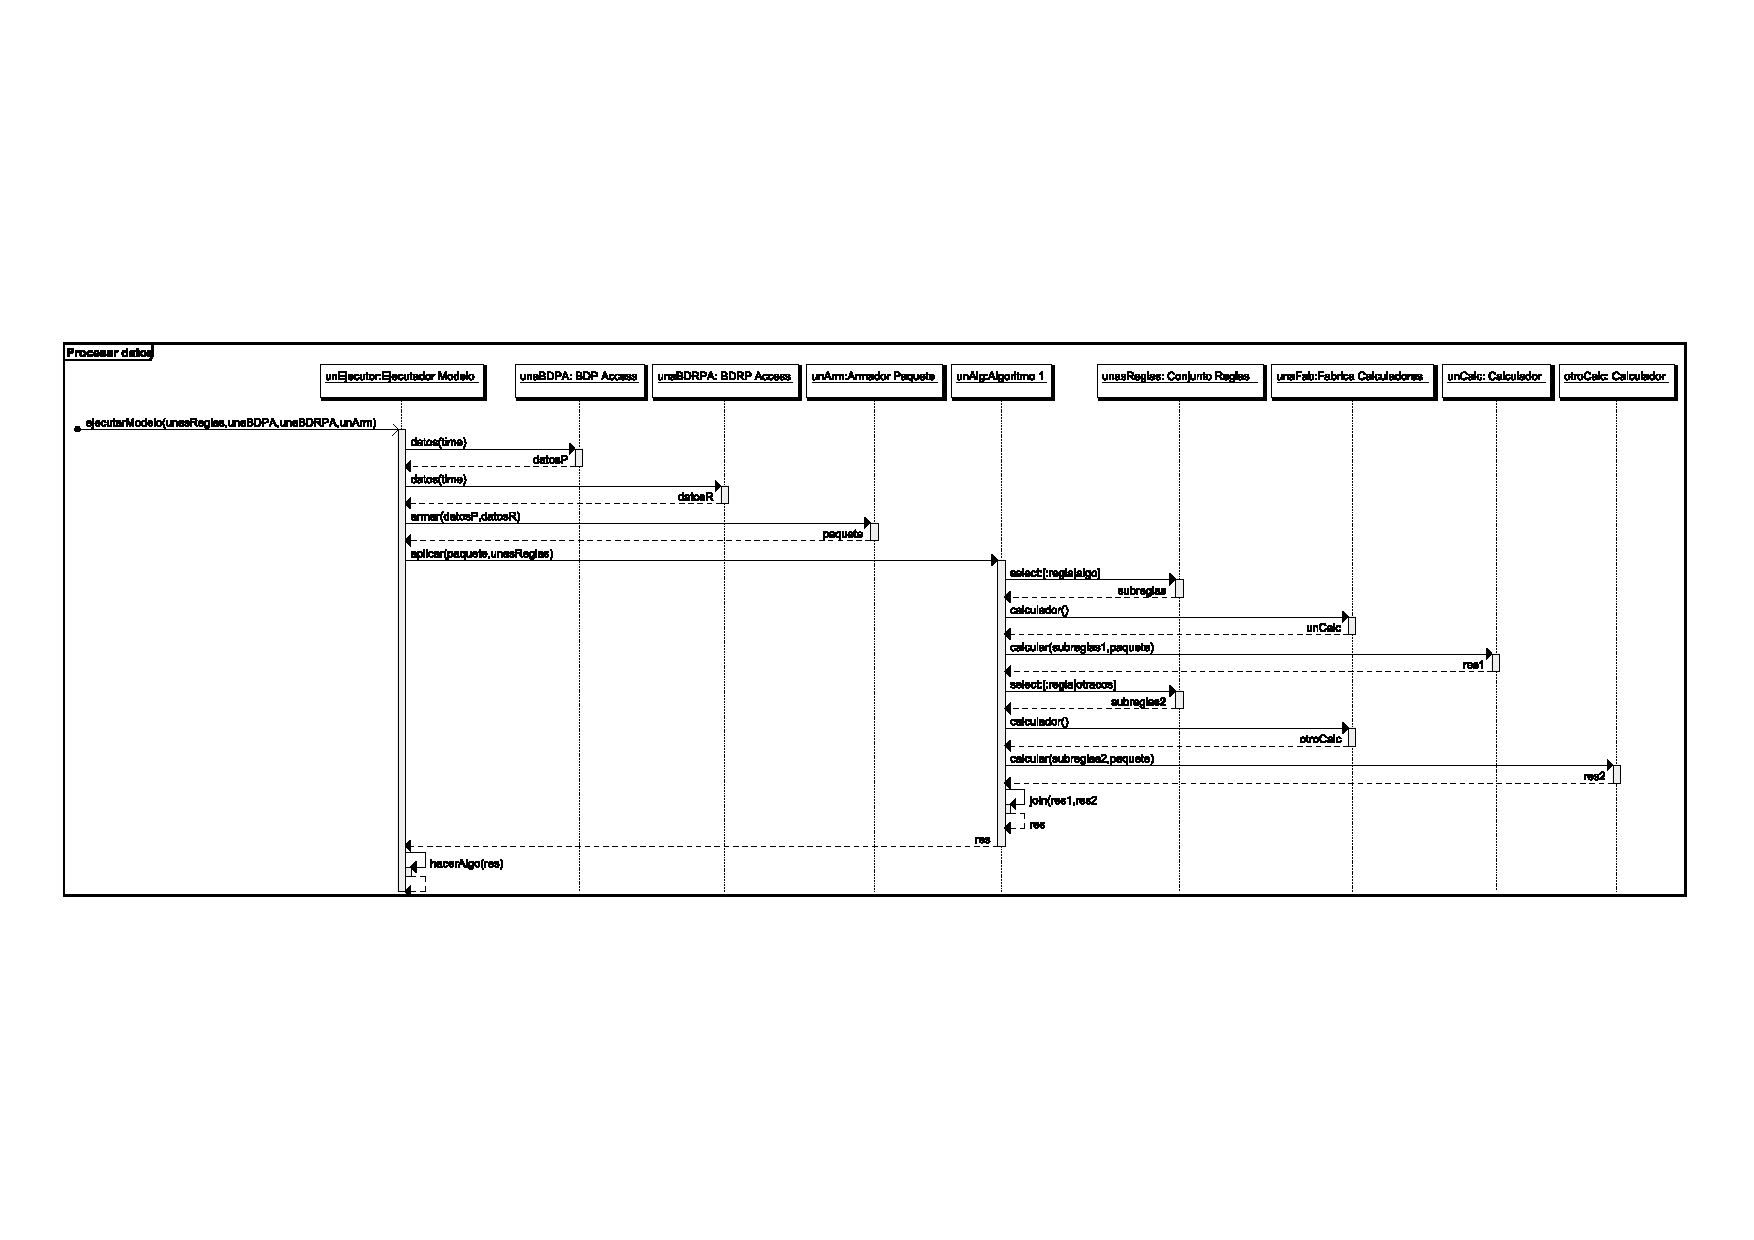
\includegraphics[scale=0.55]{../secuencias.png}
\end{figure}

\begin{figure}[h]
\centering
\includegraphics[scale=0.8]{../aplicarReglas.png}
\end{figure}

\begin{figure}[h]
\centering
\includegraphics[scale=0.7]{../creaYDestruyeCalc.png}
\end{figure}

\clearpage
\newpage
\clearpage

\newpage
\chapter{Comparaci�n UP-Scrum}

A lo largo del desarrollo hemos trabajado con dos metodolog�as de desarrollo del software: UP y Scrum. Ambas tuvieron sus comodidades y es posible distinguir para alguna de ellas ciertas dificultades.

Ambas son metodolog�as �giles de desarrollo, una basada en iteraciones, y la otra en sprints, sin embargo la caracter�stica en com�n es la idea de un desarrollo iterativo incremental del producto final.

Las diferencias se encuentran en tecnicismos sobre el modo de documentaci�n y trabajo en general. Comencemos hablando un poco de la documentaci�n. UP pone mucho �nfasis en la documentaci�n, provee templates, en muchos casos demasiado complicados y detallados en exceso para la mayor�a de los proyectos de desarrollo. Es por ello, que se adapta �sta metodolog�a de desarrollo al proyecto en que uno tiene que trabajar (la adaptaci�n est� prevista por RUP), e inclusive, un entregable o artefacto es justamente la documentaci�n de la adaptaci�n del modelo al proyecto. Esto puede hacer que uno no s�lo pierda tiempo intentando descifrar los templates sino que muchas veces no toda la documentaci�n es esencial, e incluso puede salvarse con apartados explicatorios de lo que uno va desarrollando.

Scrum tambi�n provee documentaci�n pero de una manera m�s simp�tica y f�cil no s�lo de aprender sino de comunicar a los stakeholders. En Scrum las funcionalidades se ven reflejadas en �pics, y todo requerimiento viene presentado como user stories, puestos desde la perspectiva de los clientes, y con casos de aceptaci�n que le ayudan a uno a saber si un user story est� completo o no. La idea de ponerse del lado del cliente en el desarrollo de user stories facilita m�s la noci�n de lo que uno debe hacer para satisfacer las expectativas de los mismos reflejadas en los casos de aceptaci�n.

Puede ser una tarea complicada en UP ver los requerimientos como casos de uso. En nuestro caso en particular, nos result� bastante complicado hacer un mapeo entre los mismos y las funcionalidades a implementar. En Scrum tambi�n nos result� complicado el mapeo con user stories, pero m�s que nada por la forma que ten�a el problema a tratar. Consideramos que en general es m�s f�cil trabajar con user stories que con casos de uso.

En este punto, pensamos que Scrum de adapt� mejor a nuestro trabajo, ya que est� pensado para equipo chicos (un poco m�s grandes que el nuestro, pero no tanto) mientras que RUP est� pensado como un m�todo para equipos grandes o chicos,que debe ser adaptado a la circunstancia. Entonces, Scrum no necesit� ser adaptado, como si pas� con RUP (solamente el �ndice de los templates de Rup ocupaba varias p�ginas, la documentaci�n es excesiva, en nuestra opini�n).

En cuanto a las cosas que pueden afectar a un proyecto en UP se documentan los riesgos, el impacto, la probabilidad de ocurrencia y las acciones de mitigaci�n entre otras cosas. Y se lleva a cabo el seguimiento de los mismos, intentando mitigar aquellos que son m�s urgentes y presentando entregables con dicho seguimiento.

En Scrum uno no analiza riesgos sino que considera impedimentos que puedan molestar al desarrollo. Si bien parecen nociones similares no lo son del todo, los impedimentos son removibles con las acciones adecuadas, los riesgos deben ser mitigados pero pueden seguir existiendo. Creemos que no le vendr�a mal a Scrum presentar riesgos tambi�n.

Tomemos otra rama, la planificaci�n y el seguimiento del plan. En UP se estiman los casos de uso con por ejemplo rondas de estimaci�n hasta llegar a un consenso(se pueden usar puntos de funci�n), en Scrum se estima de manera relativa, por ejemplo con los n�meros de fibonacci, y luego se hacen estimaciones de esfuerzo. Aqu� creemos que los m�todos son similares as� que en principio se pueden utilizar indistintamente sin sacarse ventajas. Lo que por ah� es m�s f�cil es el seguimiento en Scrum. Gracias a Sprint Backlog que muestra como se van adaptando las estimaciones d�a a d�a, se puede observar en el burdown chart, como va avanzando el proyecto de una manera gr�fica y mas comprensible. En UP al utilizar estimaciones iniciales uno debe analizar los desv�os. La manera m�s sencilla es mediante l�neas de base, pero podr�a tambi�n modificar el plan. Si embargo el modo de seguimiento en scrum nos parece no s�lo m�s din�mico, f�cil, r�pido y entendible sino que tambi�n, es m�s liviano de implementar. 

Es deseable hacer las daily stand up meetings que utiliza Scrum, recordemos que Brooks dec�a que un proyecto podr�a atrasarse 3 meses un d�a por vez. La idea de estas reuniones cortas y efectivas es que todos tengan idea de lo que se est� haciendo en conjunto, todos los d�as.

Tanto en Scrum como en UP aparecen los requerimientos asociados con funcionalidades como los atributos de calidad, sin embargo Scrum trata como una sola cosa a ambos requerimientos, para Scrum todo es un User Story. Consideramos que en cuanto a �sto es bueno diferenciar ambas cosas, ya que brinda mayor calidad de lectura y comprensi�n.

 
La asignaci�n de recursos es otro tema a debatir. Mientras que en UP, se planifican los recursos de antemano, s�lo se reasignan en caso de ser necesario, por lo cual la asignaci�n es bastante est�tica y carece de proyecci�n a futuro. Adem�s puede crear que se considere a una persona apta para realizar una tarea y luego no pueda. En Scrum en cambio los intengrantes del equipo se postulan a las tareas y no comienzan a hacer otra cosa hasta que la finalicen. Por otra parte como se mencion� antes el daily stand up meeting favorece ver c�mo cada uno va cumpliendo o no aquello que se propuso a realizar.

Creemos que finalmente antes �stos dos m�todos utilizados, Scrum es m�s ventajoso por su r�pidez y sencillez al momento de llevarlo a cabo, lo cual hace menos f�cil atrasarse. Scrum con algo m�s de documentaci�n podr�a convertirse en un m�todo totalmente robusto y apto para el desarrollo.
\clearpage

\newpage
\chapter{Bibliograf�a}

\item Slides de la materia sobre Scrum

\item http://www.controlchaos.com/

\item Software Architecture in Practice, Second Edition. Len Bass, Paul Clements , Rick Kazman . Addison-Wesley Professional, 2003. 
\item Documentaci�n online de Python 2.6

\end{itemize}
\clearpage

\newpage
\chapter{Conclusi�n}

Si bien se sabe que el dise�o del proyecto esta en sus primeros pasos, con lo realizado en esta preentrega, se tiene una especificaci�n relativamente exhaustiva de las cosas mas importantes del dominio del problema. Con estos datos se pudo definir la base de la arquitectura del sistema, que si bien puede cambiar, se supone que no afectara gravemente el dise�o original, ni traer� problemas que posterguen demasiado el proyecto.

Para realizar esta afirmaci�n nos basamos en que al realizar el diagrama contextual (que sirve en este caso de arquitectura), tomamos en cuenta varios de los requerimientos y atributos de calidad planteados inicialmente, proponiendo una arquitectura que es incremental, en cuanto a que se pueden agregar Terminales Remotas, y en cuanto a que se puede incrementar el poder de computo. Tambi�n es resistente a fallas en las transmisiones, ya que se implementara un protocolo confiable entre las TRs y la Estaci�n Central y tambi�n es resistente a fallas en los equipos, dado que se van a poder subsanar la caida de una TR triangulando o utilizando un servicio externo. Adem�s se contempla el hecho de tener comunicaci�n con diferente tipo de sistemas, ya sean clientes externos (como AgroTop), proveedores de servicio (Biggest Satelite) y usuarios internos, encargados de monitorear el estado del sistema.

Adem�s de todo esto se dise�o un plan que tiene en cuenta tiempos de entrega y de desarrollo que son acotados, por esta raz�n se tuvo que identificar dependencias entre las funcionalidades principales que se detectaron, como as� su importancia y complejidad dentro del sistema.

Como se conoce estos m�todos llevan bastante tiempo, pero ayudan a tener un control del proyecto y tener luego un hilo de ejecuci�n bien definido que permitir� optimizar el desarrollo del sistema durante el tiempo. Teniendo en cuenta el contexto en el que se realizo el trabajo creemos haber cumplido las expectativas en cuanto a los requerimientos pedidos para esta entrega.

\clearpage
\label{LastPage}
\end{document}
